\documentclass{book}
\usepackage[paperwidth=148mm,paperheight=55mm,text={148mm,160mm},left=0mm,top=10pt]{geometry}
\usepackage{ctexcap}
\usepackage[labelfont=bf,labelsep=quad]{caption}
  \DeclareCaptionFont{kai}{\kaishu}
  \captionsetup{textfont=kai}
\usepackage{graphicx,floatrow,subfig}
\renewcommand{\rmdefault}{ptm}
\begin{document}
\setcounter{chapter}{2}

\begin{figure}[!h]
\ffigbox[\FBwidth]{}{%
\begin{subfloatrow}[3]
\ffigbox[1.5\FBwidth]{\caption{���ε�Ч��·}}{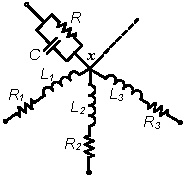
\includegraphics{fig36.pdf}}
\ffigbox[1.5\FBwidth]{\caption{�Ķ˵�Ч��·}}{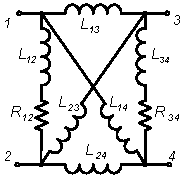
\includegraphics{fig35.pdf}}
\ffigbox[1.5\FBwidth]{\caption{�����ε�Ч��· }}{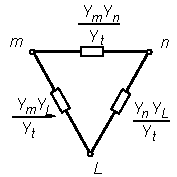
\includegraphics{fig43.pdf}}
\end{subfloatrow}
\caption{SRR �����ֵ�Ч��·ͼ}}
\end{figure}
\end{document}
